\documentclass[a4paper,twoside,11pt]{article}
\usepackage{a4wide,graphicx,fancyhdr,clrscode,tabularx,amsmath,amssymb,color,enumitem, subfig}

\usepackage[english]{isodate}

%----------------------- Macros and Definitions --------------------------

\setlength\headheight{20pt}
\addtolength\topmargin{-10pt}
\addtolength\footskip{20pt}

\fancypagestyle{plain}{%
\fancyhf{}
\fancyhead[LO,RE]{\sffamily AE 706}
\fancyhead[RO,LE]{\sffamily Computational Fluid Dynamics}
\fancyfoot[RO,LE]{\sffamily\bfseries\thepage}
\renewcommand{\headrulewidth}{0pt}
\renewcommand{\footrulewidth}{0pt}
}

\pagestyle{fancy}
\fancyhf{}
\fancyhead[LO,RE]{\sffamily Computational Fluid Dynamics}
\fancyhead[RO,LE]{\sffamily AE 706}
\fancyfoot[RO,LE]{\sffamily\bfseries\thepage}
\renewcommand{\headrulewidth}{0pt}
\renewcommand{\footrulewidth}{0pt}

\newcommand{\R}{{\mathbb R}}
\newcommand{\N}{{\mathbb N}}
\newcommand{\Z}{{\mathbb Z}}
\newcommand{\Q}{{\mathbb Q}}

\begin{document}


\title{\vspace{-2\baselineskip}
Assignment 1 Report}
\author{Amal S Sebastian \\ {170010054}}

\maketitle


The assignment requires us to solve the 1 dimensional advection equation (positive a) given a set of initial conditions, using different numerical schemes. Given below are the results obtained for all schemes, general observations are made at the end of each scheme.


\subsection*{FTFS Scheme}
\begin{table}[h]
    \centering
    \begin{tabular}{ | c | m{5cm} | m{5cm} | }
      \hline
      \begin{minipage}{.3\textwidth}
        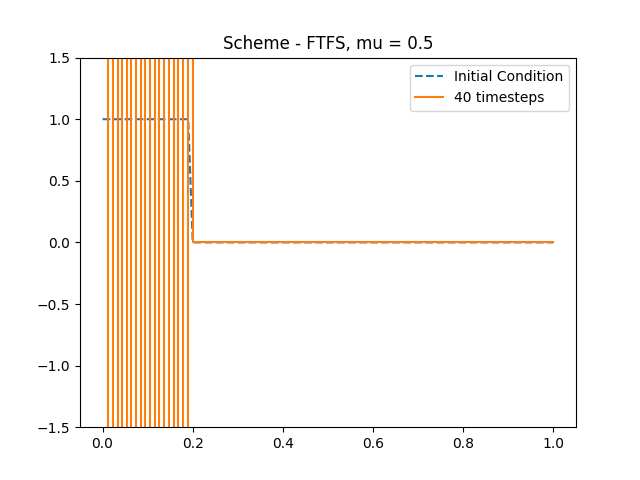
\includegraphics[width=\linewidth, height=2.75cm]{../plots/scheme1-IC1-mu0_5.png}
      \end{minipage}
      &
      \begin{minipage}{.3\textwidth}
        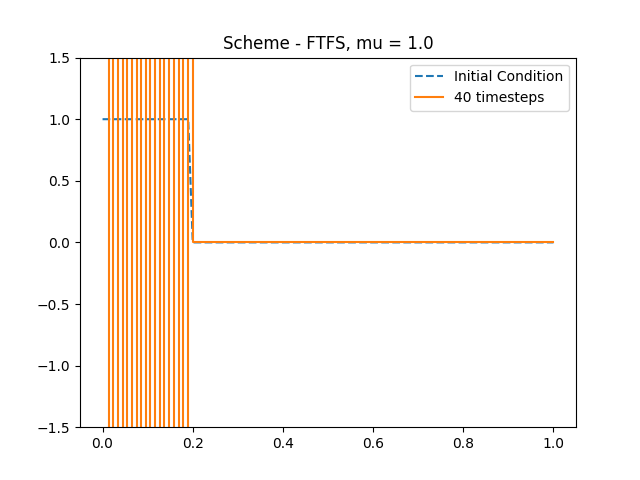
\includegraphics[width=\linewidth, height=2.75cm]{../plots/scheme1-IC1-mu1_0.png}
      \end{minipage}
      &
      \begin{minipage}{.3\textwidth}
        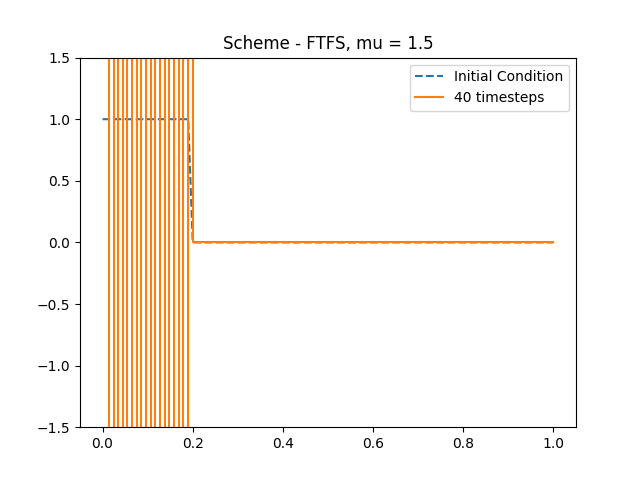
\includegraphics[width=\linewidth, height=2.75cm]{../plots/scheme1-IC1-mu1_5.png}
      \end{minipage} \\
      \begin{minipage}{.3\textwidth}
        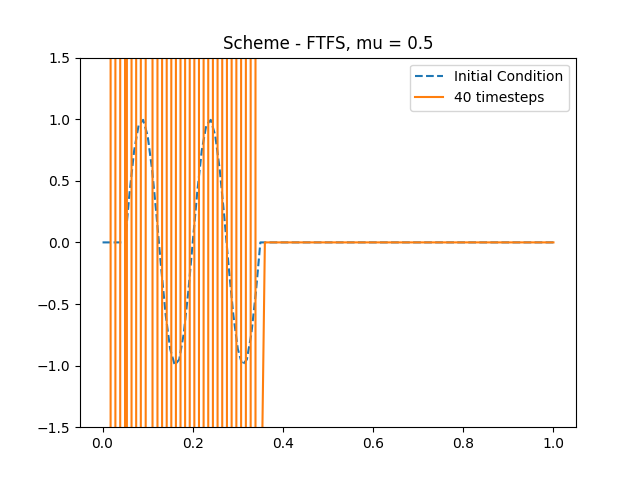
\includegraphics[width=\linewidth, height=2.75cm]{../plots/scheme1-IC2-mu0_5.png}
      \end{minipage}
      &
      \begin{minipage}{.3\textwidth}
        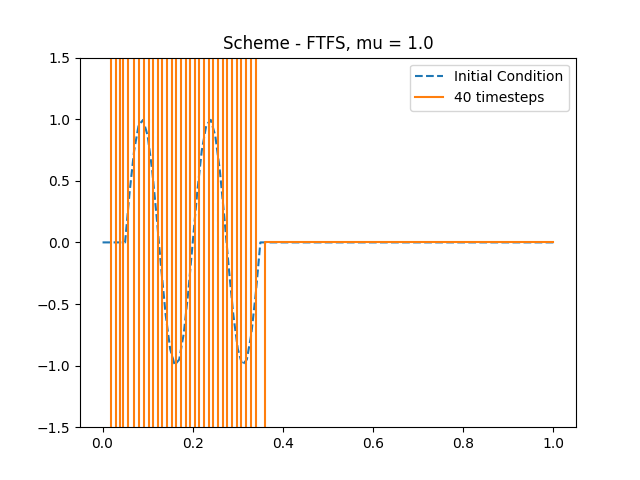
\includegraphics[width=\linewidth, height=2.75cm]{../plots/scheme1-IC2-mu1_0.png}
      \end{minipage}
      &
      \begin{minipage}{.3\textwidth}
        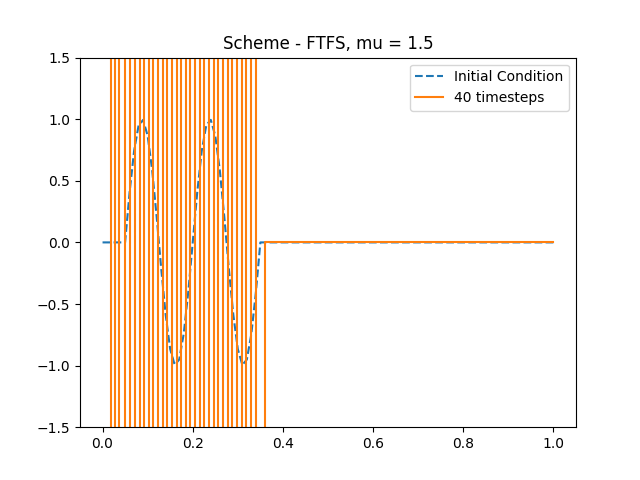
\includegraphics[width=\linewidth, height=2.75cm]{../plots/scheme1-IC2-mu1_5.png}
      \end{minipage} \\
      \begin{minipage}{.3\textwidth}
        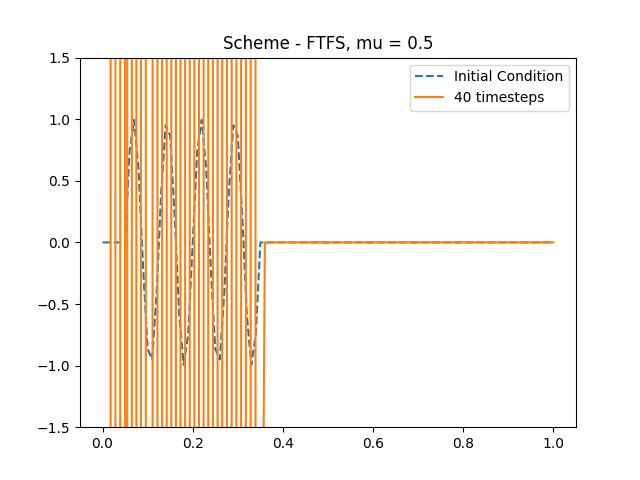
\includegraphics[width=\linewidth, height=2.75cm]{../plots/scheme1-IC3-mu0_5.png}
      \end{minipage}
      &
      \begin{minipage}{.3\textwidth}
        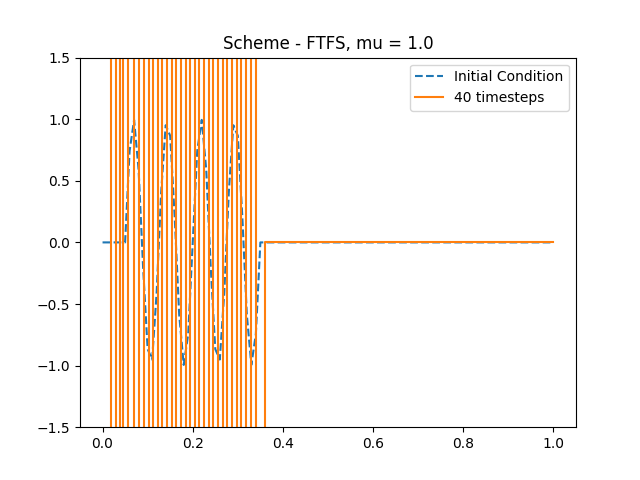
\includegraphics[width=\linewidth, height=2.75cm]{../plots/scheme1-IC3-mu1_0.png}
      \end{minipage}
      &
      \begin{minipage}{.3\textwidth}
        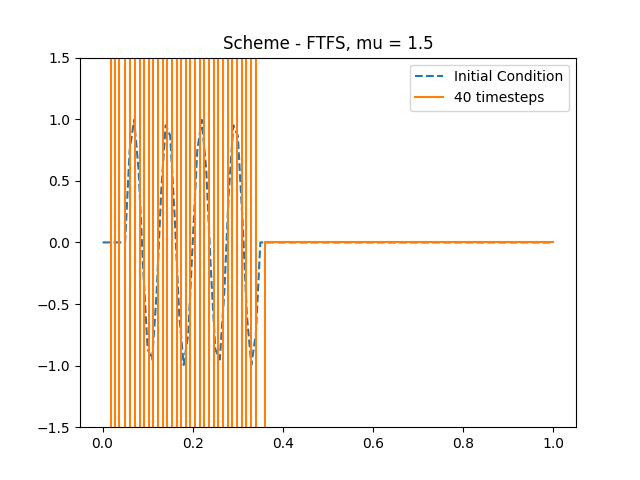
\includegraphics[width=\linewidth, height=2.75cm]{../plots/scheme1-IC3-mu1_5.png}
      \end{minipage} \\
      \begin{minipage}{.3\textwidth}
        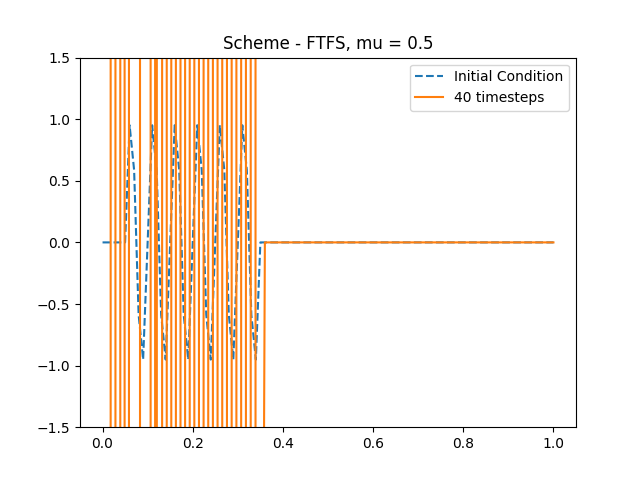
\includegraphics[width=\linewidth, height=2.75cm]{../plots/scheme1-IC4-mu0_5.png}
      \end{minipage}
      &
      \begin{minipage}{.3\textwidth}
        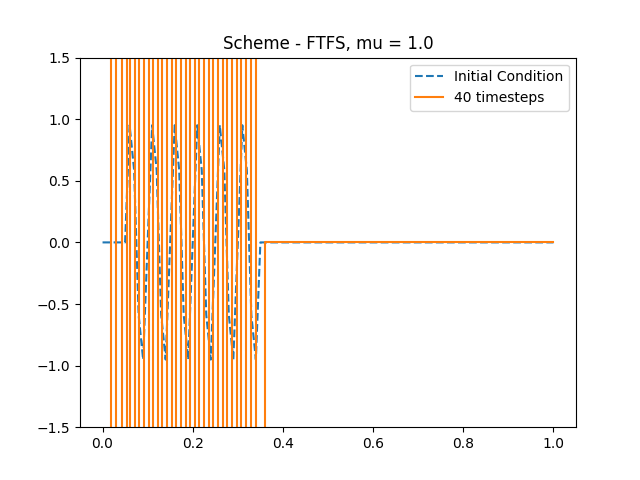
\includegraphics[width=\linewidth, height=2.75cm]{../plots/scheme1-IC4-mu1_0.png}
      \end{minipage}
      &
      \begin{minipage}{.3\textwidth}
        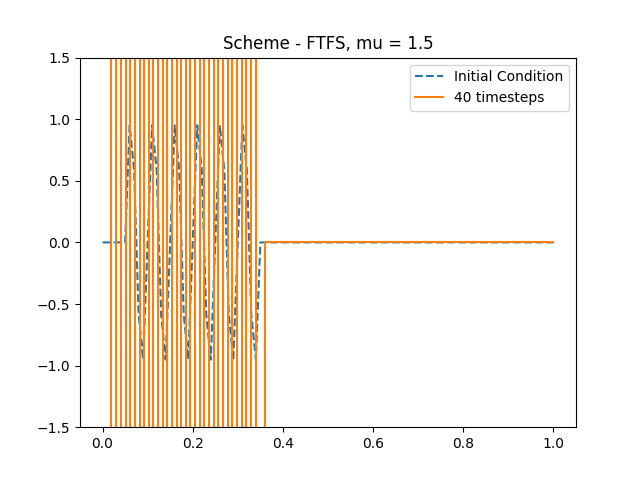
\includegraphics[width=\linewidth, height=2.75cm]{../plots/scheme1-IC4-mu1_5.png}
      \end{minipage} \\
      \begin{minipage}{.3\textwidth}
        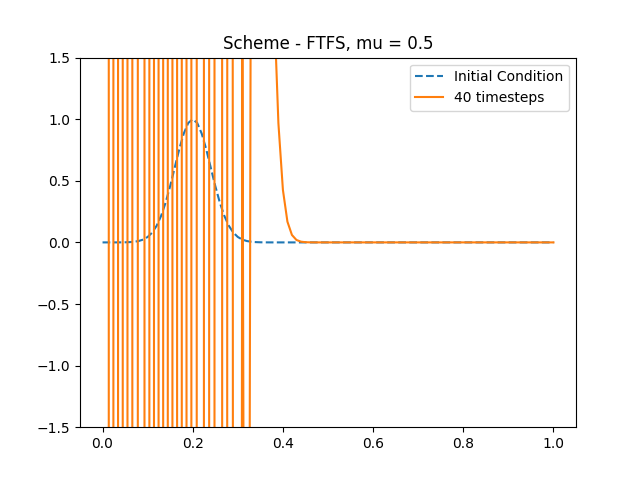
\includegraphics[width=\linewidth, height=2.75cm]{../plots/scheme1-IC5-mu0_5.png}
      \end{minipage}
      &
      \begin{minipage}{.3\textwidth}
        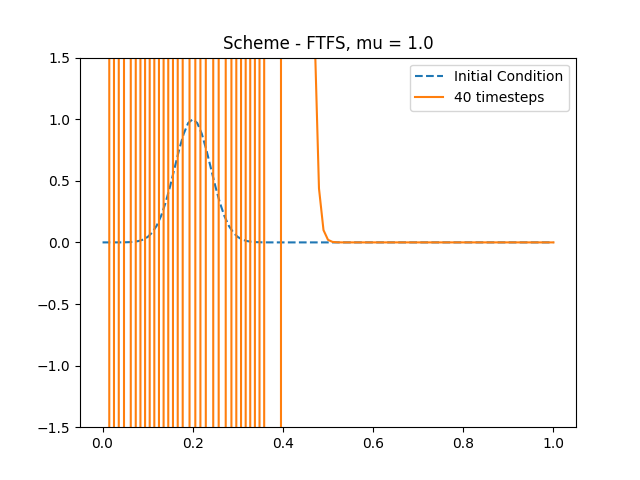
\includegraphics[width=\linewidth, height=2.75cm]{../plots/scheme1-IC5-mu1_0.png}
      \end{minipage}
      &
      \begin{minipage}{.3\textwidth}
        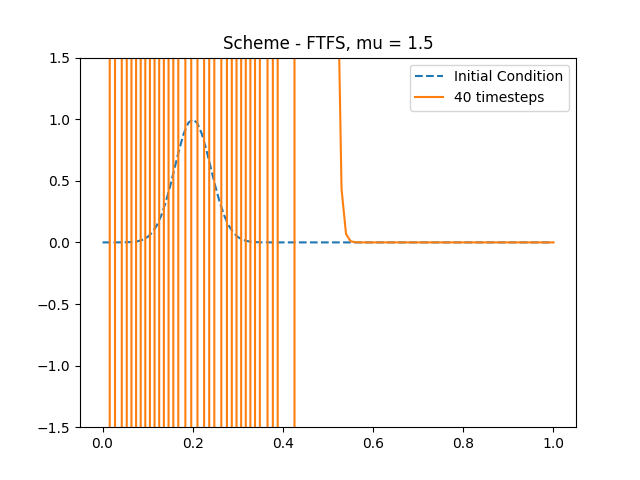
\includegraphics[width=\linewidth, height=2.75cm]{../plots/scheme1-IC5-mu1_5.png}
      \end{minipage} \\
      \hline
    \end{tabular}
  \end{table}

All initial conditions for all CFL numbers are unstable using the FTFS scheme.


\newpage
  \subsection*{FTCS Scheme}
  \begin{table}[!h]
      \centering
      \begin{tabular}{ | c | m{5cm} | m{5cm} | }
        \hline
        \begin{minipage}{.3\textwidth}
          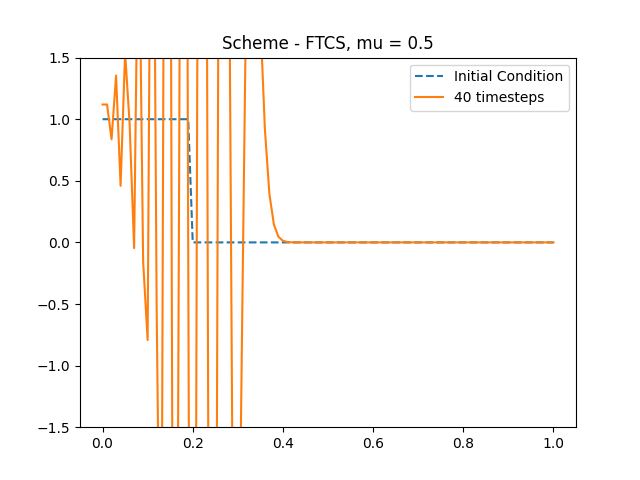
\includegraphics[width=\linewidth, height=3.5cm]{../plots/scheme2-IC1-mu0_5.png}
        \end{minipage}
        &
        \begin{minipage}{.3\textwidth}
          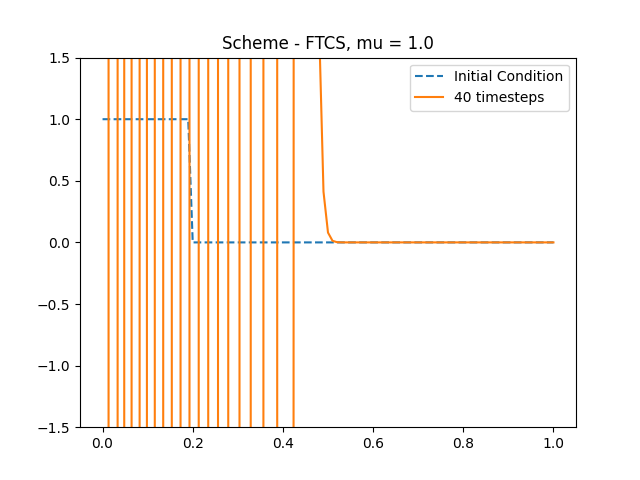
\includegraphics[width=\linewidth, height=3.5cm]{../plots/scheme2-IC1-mu1_0.png}
        \end{minipage}
        &
        \begin{minipage}{.3\textwidth}
          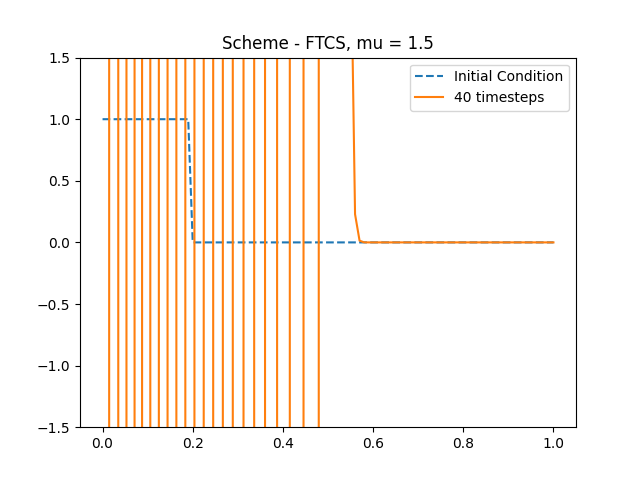
\includegraphics[width=\linewidth, height=3.5cm]{../plots/scheme2-IC1-mu1_5.png}
        \end{minipage} \\
        \begin{minipage}{.3\textwidth}
          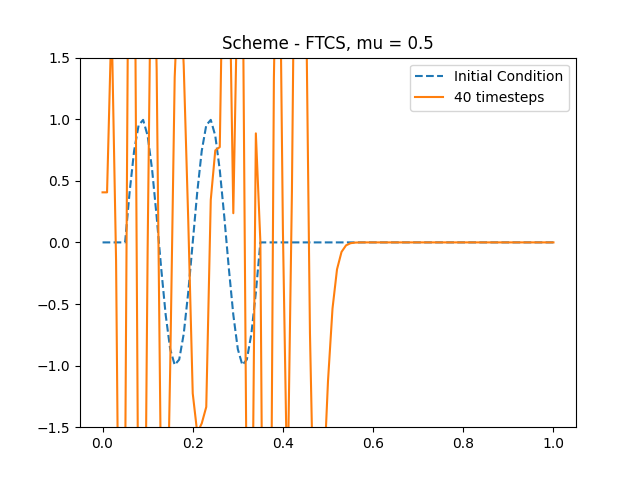
\includegraphics[width=\linewidth, height=3.5cm]{../plots/scheme2-IC2-mu0_5.png}
        \end{minipage}
        &
        \begin{minipage}{.3\textwidth}
          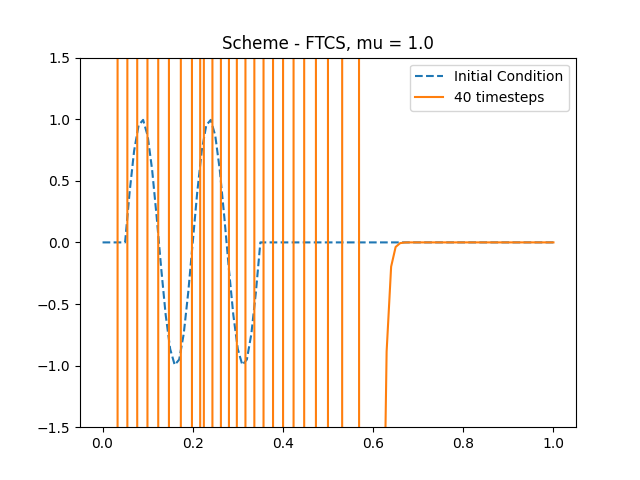
\includegraphics[width=\linewidth, height=3.5cm]{../plots/scheme2-IC2-mu1_0.png}
        \end{minipage}
        &
        \begin{minipage}{.3\textwidth}
          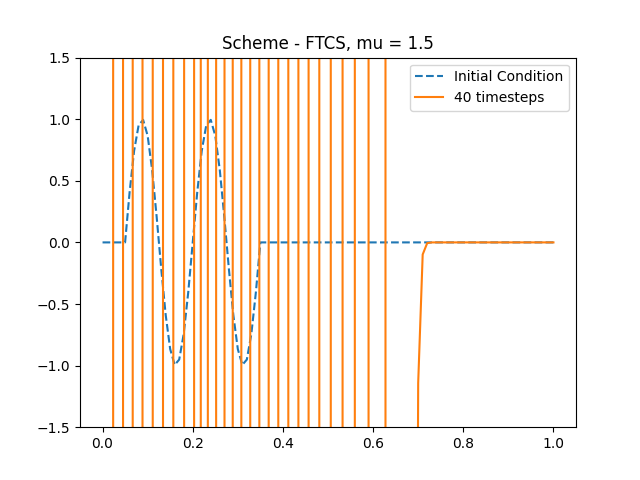
\includegraphics[width=\linewidth, height=3.5cm]{../plots/scheme2-IC2-mu1_5.png}
        \end{minipage} \\
        \begin{minipage}{.3\textwidth}
          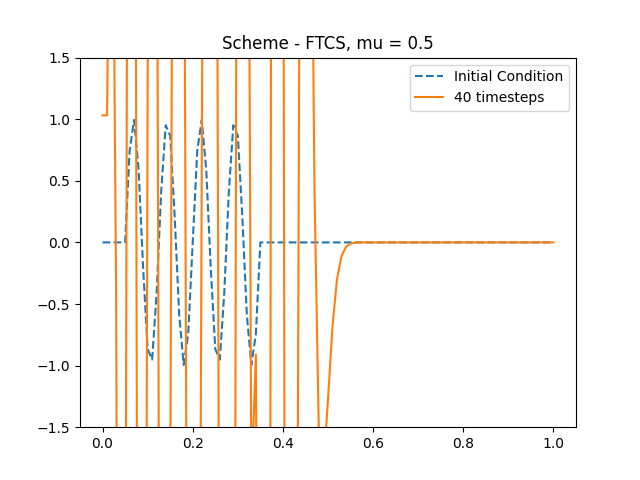
\includegraphics[width=\linewidth, height=3.5cm]{../plots/scheme2-IC3-mu0_5.png}
        \end{minipage}
        &
        \begin{minipage}{.3\textwidth}
          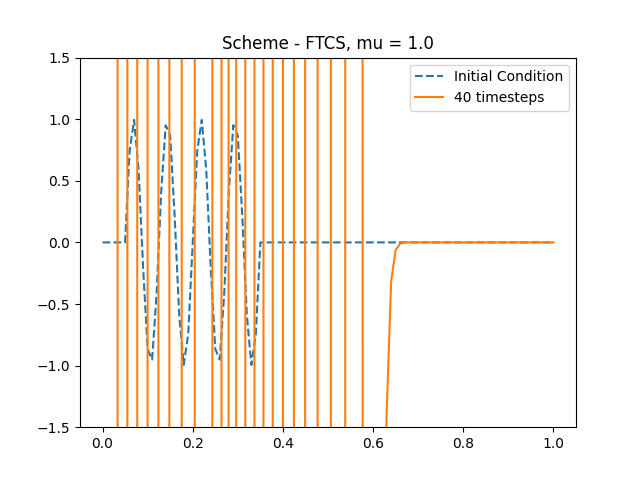
\includegraphics[width=\linewidth, height=3.5cm]{../plots/scheme2-IC3-mu1_0.png}
        \end{minipage}
        &
        \begin{minipage}{.3\textwidth}
          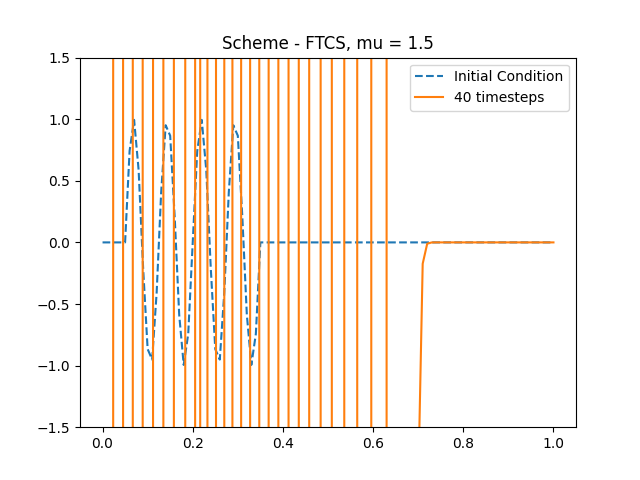
\includegraphics[width=\linewidth, height=3.5cm]{../plots/scheme2-IC3-mu1_5.png}
        \end{minipage} \\
        \begin{minipage}{.3\textwidth}
          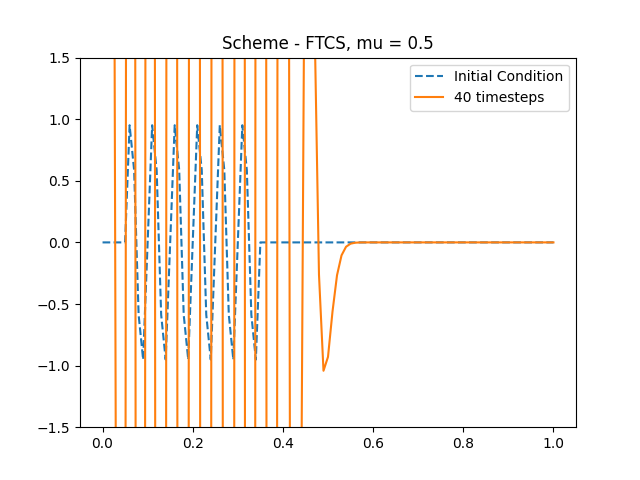
\includegraphics[width=\linewidth, height=3.5cm]{../plots/scheme2-IC4-mu0_5.png}
        \end{minipage}
        &
        \begin{minipage}{.3\textwidth}
          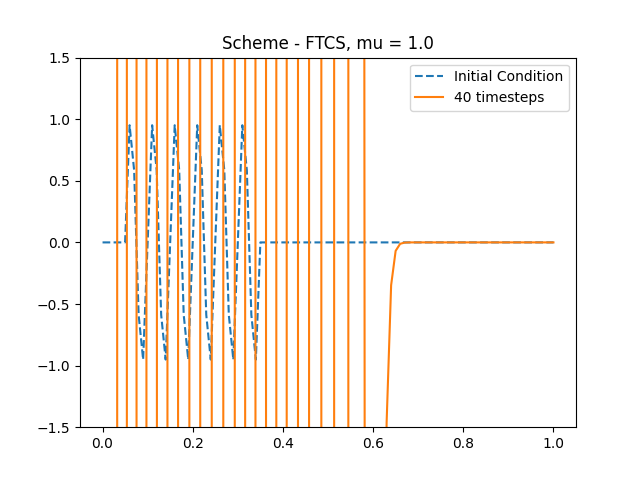
\includegraphics[width=\linewidth, height=3.5cm]{../plots/scheme2-IC4-mu1_0.png}
        \end{minipage}
        &
        \begin{minipage}{.3\textwidth}
          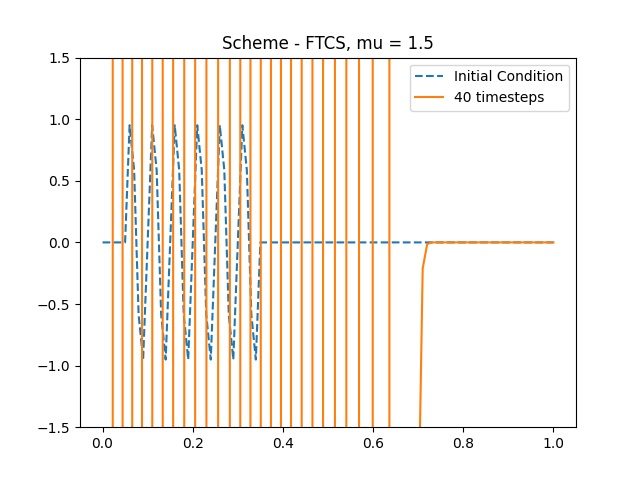
\includegraphics[width=\linewidth, height=3.5cm]{../plots/scheme2-IC4-mu1_5.png}
        \end{minipage} \\
        \begin{minipage}{.3\textwidth}
          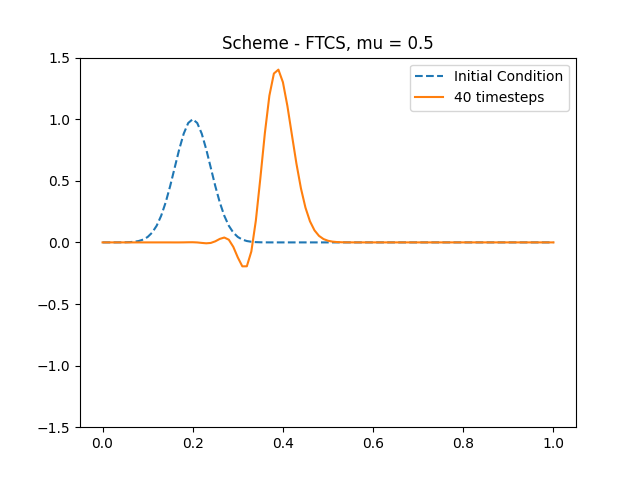
\includegraphics[width=\linewidth, height=3.5cm]{../plots/scheme2-IC5-mu0_5.png}
        \end{minipage}
        &
        \begin{minipage}{.3\textwidth}
          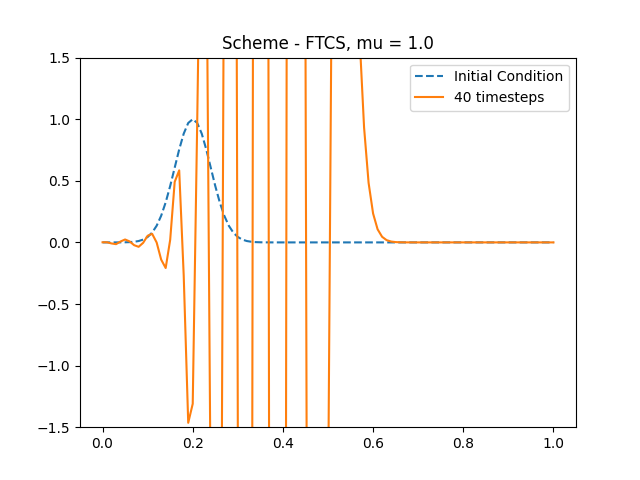
\includegraphics[width=\linewidth, height=3.5cm]{../plots/scheme2-IC5-mu1_0.png}
        \end{minipage}
        &
        \begin{minipage}{.3\textwidth}
          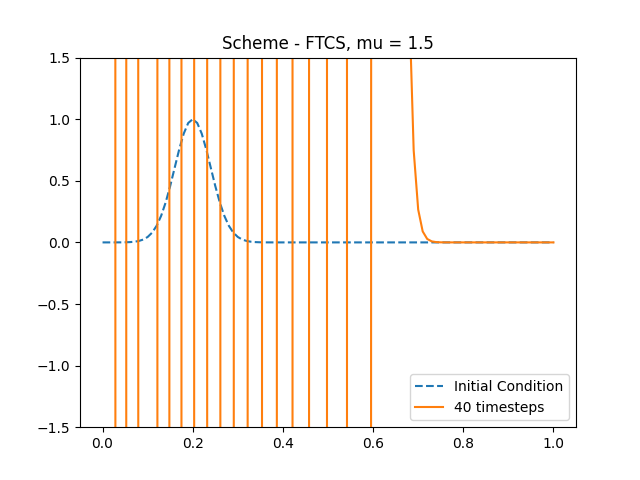
\includegraphics[width=\linewidth, height=3.5cm]{../plots/scheme2-IC5-mu1_5.png}
        \end{minipage} \\
        \hline
      \end{tabular}
    \end{table}

    We see that the FTCS scheme is also unstable for almost all initial conditions and CFL numbers. For the Gaussian initial condition with CFL number of 0.5 we see that after 40 timesteps the peak of the solution is higher than the initial condition, suggesting that this will also blow up after some more time steps.

    \newpage
    \subsection*{FTBS Scheme}
    \begin{table}[!h]
        \centering
        \begin{tabular}{ | c | m{5cm} | m{5cm} | }
          \hline
          \begin{minipage}{.3\textwidth}
            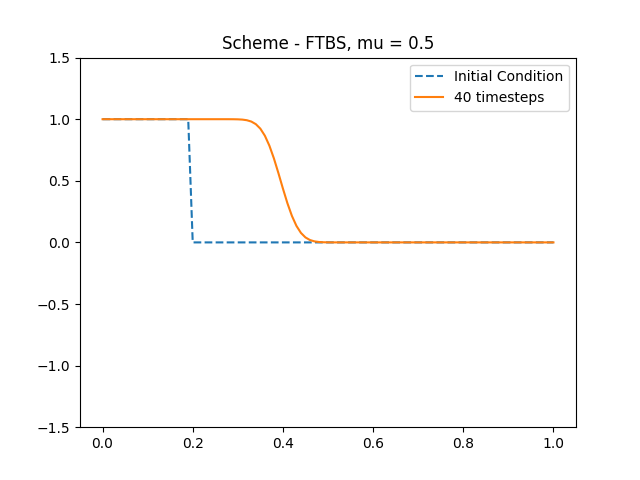
\includegraphics[width=\linewidth, height=3.5cm]{../plots/scheme3-IC1-mu0_5.png}
          \end{minipage}
          &
          \begin{minipage}{.3\textwidth}
            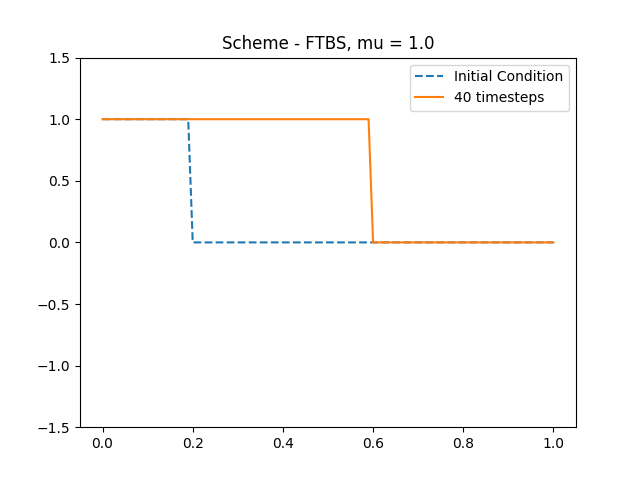
\includegraphics[width=\linewidth, height=3.5cm]{../plots/scheme3-IC1-mu1_0.png}
          \end{minipage}
          &
          \begin{minipage}{.3\textwidth}
            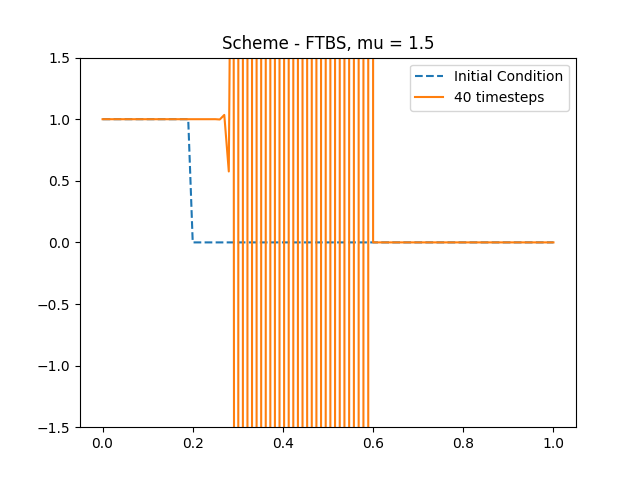
\includegraphics[width=\linewidth, height=3.5cm]{../plots/scheme3-IC1-mu1_5.png}
          \end{minipage} \\
          \begin{minipage}{.3\textwidth}
            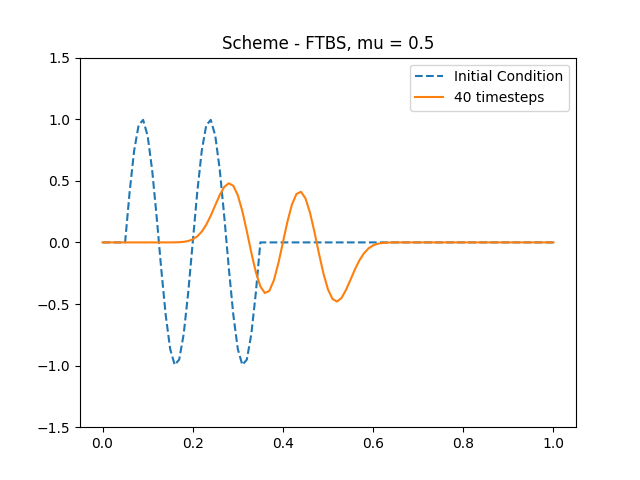
\includegraphics[width=\linewidth, height=3.5cm]{../plots/scheme3-IC2-mu0_5.png}
          \end{minipage}
          &
          \begin{minipage}{.3\textwidth}
            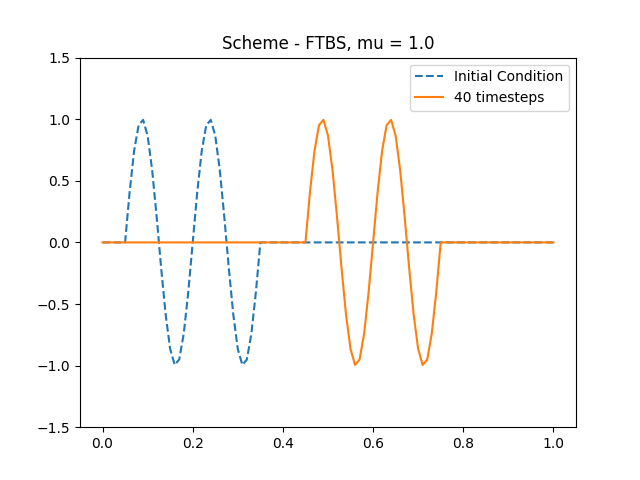
\includegraphics[width=\linewidth, height=3.5cm]{../plots/scheme3-IC2-mu1_0.png}
          \end{minipage}
          &
          \begin{minipage}{.3\textwidth}
            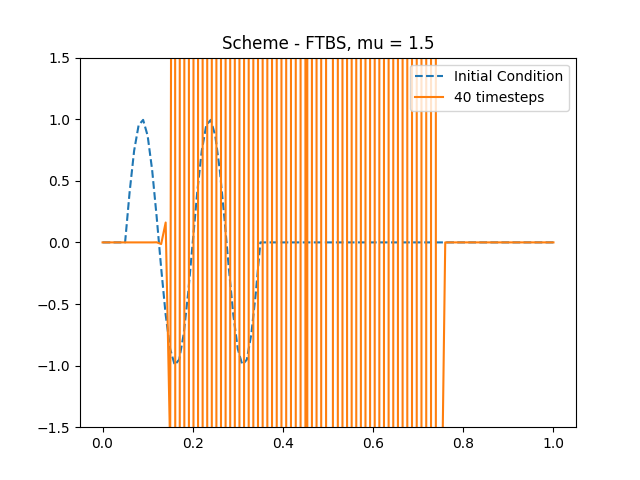
\includegraphics[width=\linewidth, height=3.5cm]{../plots/scheme3-IC2-mu1_5.png}
          \end{minipage} \\
          \begin{minipage}{.3\textwidth}
            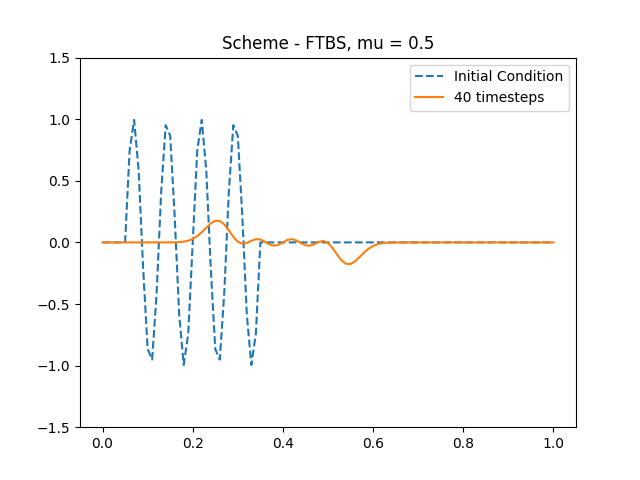
\includegraphics[width=\linewidth, height=3.5cm]{../plots/scheme3-IC3-mu0_5.png}
          \end{minipage}
          &
          \begin{minipage}{.3\textwidth}
            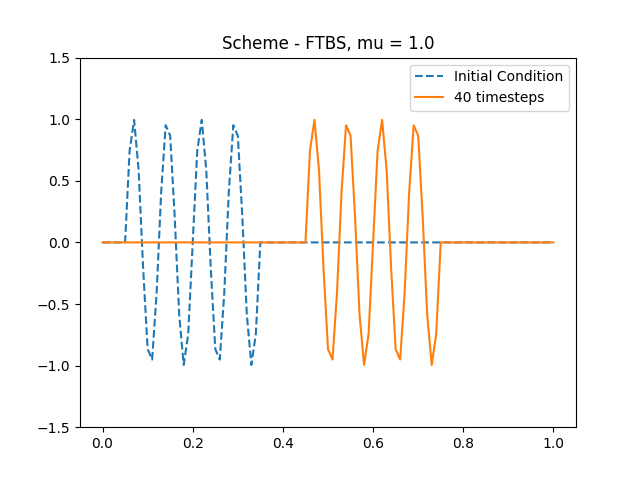
\includegraphics[width=\linewidth, height=3.5cm]{../plots/scheme3-IC3-mu1_0.png}
          \end{minipage}
          &
          \begin{minipage}{.3\textwidth}
            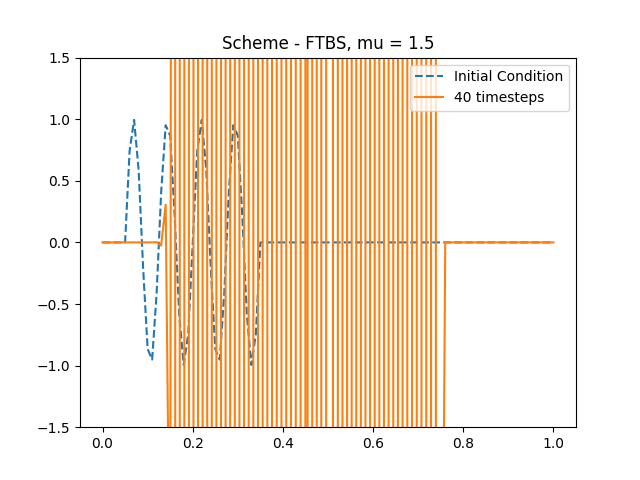
\includegraphics[width=\linewidth, height=3.5cm]{../plots/scheme3-IC3-mu1_5.png}
          \end{minipage} \\
          \begin{minipage}{.3\textwidth}
            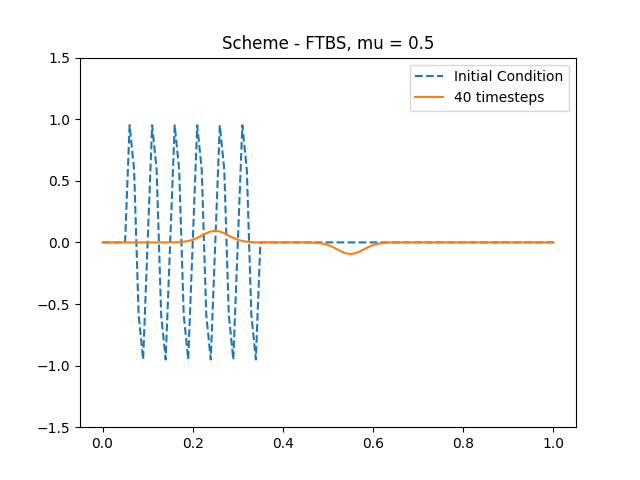
\includegraphics[width=\linewidth, height=3.5cm]{../plots/scheme3-IC4-mu0_5.png}
          \end{minipage}
          &
          \begin{minipage}{.3\textwidth}
            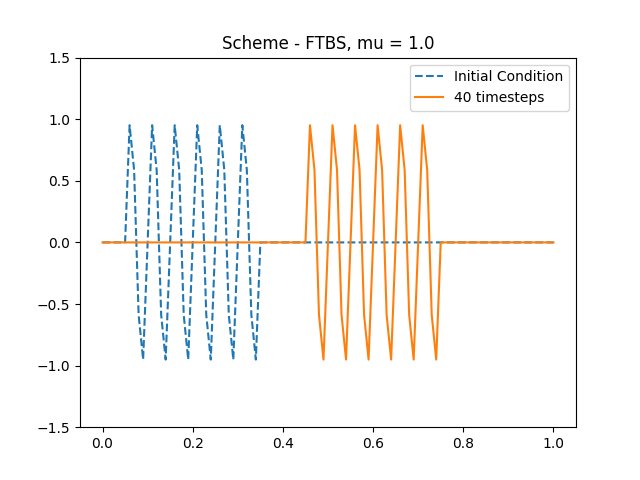
\includegraphics[width=\linewidth, height=3.5cm]{../plots/scheme3-IC4-mu1_0.png}
          \end{minipage}
          &
          \begin{minipage}{.3\textwidth}
            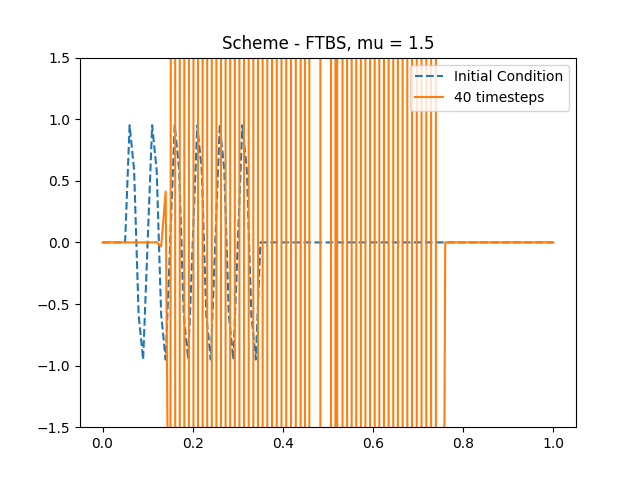
\includegraphics[width=\linewidth, height=3.5cm]{../plots/scheme3-IC4-mu1_5.png}
          \end{minipage} \\
          \begin{minipage}{.3\textwidth}
            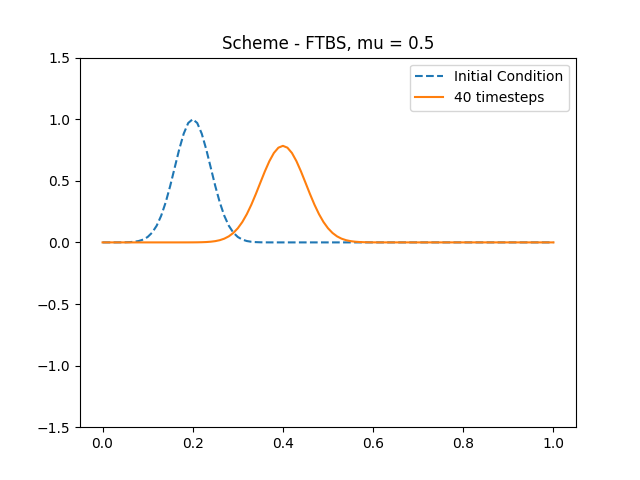
\includegraphics[width=\linewidth, height=3.5cm]{../plots/scheme3-IC5-mu0_5.png}
          \end{minipage}
          &
          \begin{minipage}{.3\textwidth}
            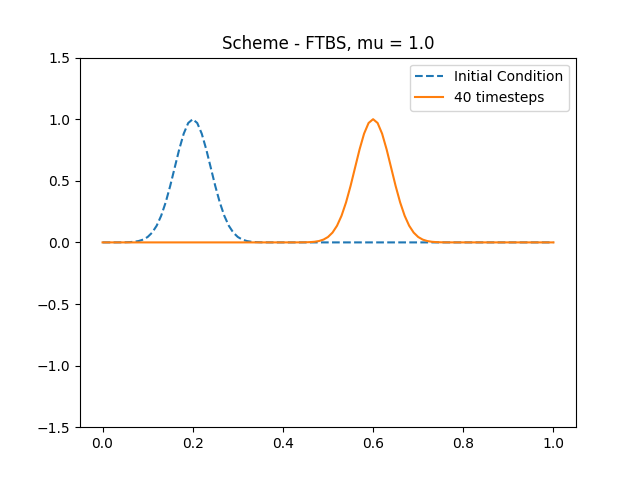
\includegraphics[width=\linewidth, height=3.5cm]{../plots/scheme3-IC5-mu1_0.png}
          \end{minipage}
          &
          \begin{minipage}{.3\textwidth}
            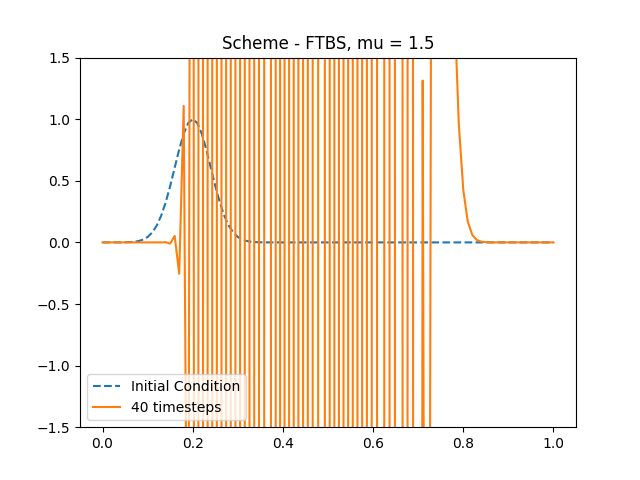
\includegraphics[width=\linewidth, height=3.5cm]{../plots/scheme3-IC5-mu1_5.png}
          \end{minipage} \\
          \hline
        \end{tabular}
      \end{table}

    We see that the FTBS scheme is unstable for all initial conditions for CFL number of 1.5.

    For CFL number = 1.0, we see that the FTBS scheme captures the exact solution accurately with no change in the wave height.

    For CFL = 0.5, we observe that the wave propagates forward however there is a decrement in the amplitude of the wave.

      \newpage
      \subsection*{LW Scheme}
      \begin{table}[!h]
          \centering
          \begin{tabular}{ | c | m{5cm} | m{5cm} | }
            \hline
            \begin{minipage}{.3\textwidth}
              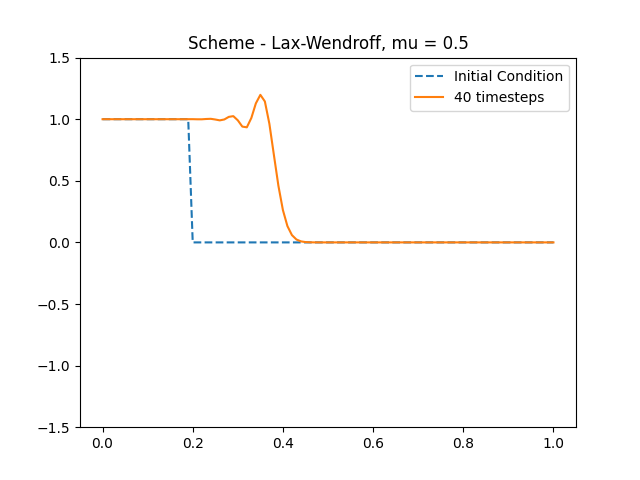
\includegraphics[width=\linewidth, height=3.5cm]{../plots/scheme4-IC1-mu0_5.png}
            \end{minipage}
            &
            \begin{minipage}{.3\textwidth}
              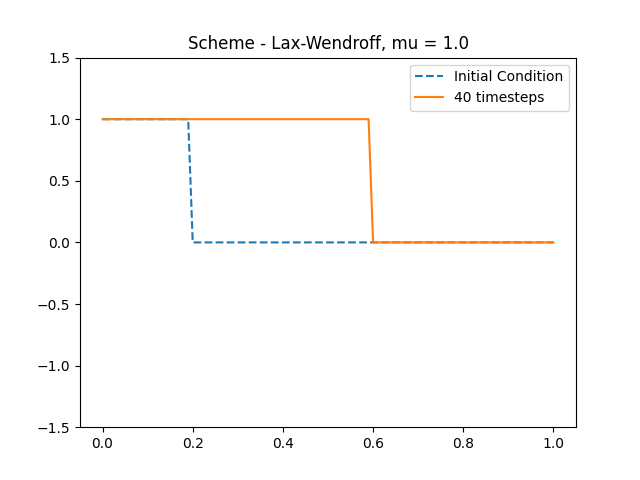
\includegraphics[width=\linewidth, height=3.5cm]{../plots/scheme4-IC1-mu1_0.png}
            \end{minipage}
            &
            \begin{minipage}{.3\textwidth}
              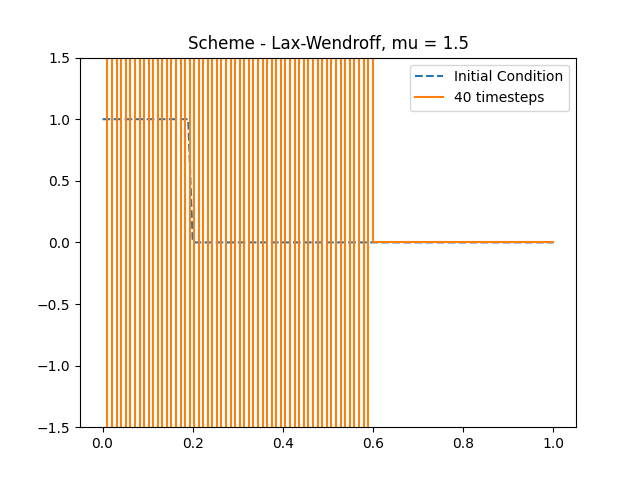
\includegraphics[width=\linewidth, height=3.5cm]{../plots/scheme4-IC1-mu1_5.png}
            \end{minipage} \\
            \begin{minipage}{.3\textwidth}
              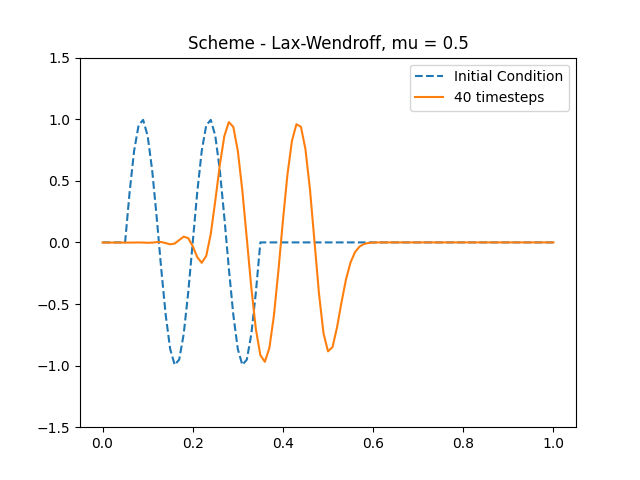
\includegraphics[width=\linewidth, height=3.5cm]{../plots/scheme4-IC2-mu0_5.png}
            \end{minipage}
            &
            \begin{minipage}{.3\textwidth}
              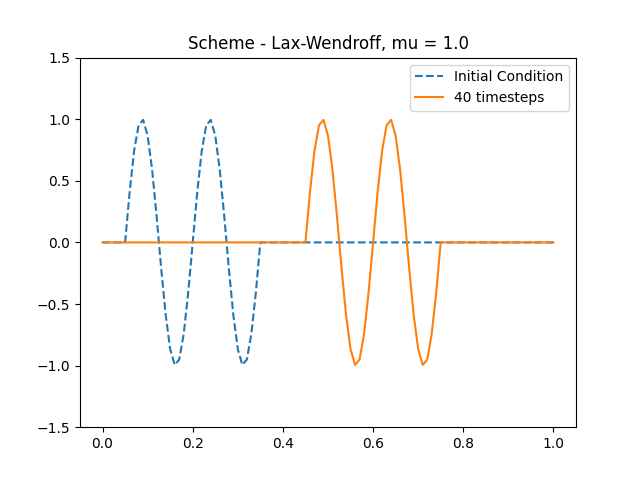
\includegraphics[width=\linewidth, height=3.5cm]{../plots/scheme4-IC2-mu1_0.png}
            \end{minipage}
            &
            \begin{minipage}{.3\textwidth}
              \includegraphics[width=\linewidth, height=3.5cm]{../plots/scheme4-IC2-mu1_5.png}
            \end{minipage} \\
            \begin{minipage}{.3\textwidth}
              \includegraphics[width=\linewidth, height=3.5cm]{../plots/scheme4-IC3-mu0_5.png}
            \end{minipage}
            &
            \begin{minipage}{.3\textwidth}
              \includegraphics[width=\linewidth, height=3.5cm]{../plots/scheme4-IC3-mu1_0.png}
            \end{minipage}
            &
            \begin{minipage}{.3\textwidth}
              \includegraphics[width=\linewidth, height=3.5cm]{../plots/scheme4-IC3-mu1_5.png}
            \end{minipage} \\
            \begin{minipage}{.3\textwidth}
              \includegraphics[width=\linewidth, height=3.5cm]{../plots/scheme4-IC4-mu0_5.png}
            \end{minipage}
            &
            \begin{minipage}{.3\textwidth}
              \includegraphics[width=\linewidth, height=3.5cm]{../plots/scheme4-IC4-mu1_0.png}
            \end{minipage}
            &
            \begin{minipage}{.3\textwidth}
              \includegraphics[width=\linewidth, height=3.5cm]{../plots/scheme4-IC4-mu1_5.png}
            \end{minipage} \\
            \begin{minipage}{.3\textwidth}
              \includegraphics[width=\linewidth, height=3.5cm]{../plots/scheme4-IC5-mu0_5.png}
            \end{minipage}
            &
            \begin{minipage}{.3\textwidth}
              \includegraphics[width=\linewidth, height=3.5cm]{../plots/scheme4-IC5-mu1_0.png}
            \end{minipage}
            &
            \begin{minipage}{.3\textwidth}
              \includegraphics[width=\linewidth, height=3.5cm]{../plots/scheme4-IC5-mu1_5.png}
            \end{minipage} \\
            \hline
          \end{tabular}
        \end{table}

    For CFL = 1.5, for all initial conditions the solution blows up.

    For CFL = 1.0, we capture the exact solution for all initial conditions.

    For CFL = 0.5, we get solutions which propagate forwards however the amplitude of the solutions decreases. The also observe in the step function initial condition that there is some distortion in the solution where we expect the vertical drop. The Gaussian initial condition however looks to be unaffected for stable CFL numbers.

      \newpage
      \subsection*{BW Scheme}
      \begin{table}[!h]
          \centering
          \begin{tabular}{ | c | m{5cm} | m{5cm} | }
            \hline
            \begin{minipage}{.3\textwidth}
              \includegraphics[width=\linewidth, height=3.5cm]{../plots/scheme5-IC1-mu0_5.png}
            \end{minipage}
            &
            \begin{minipage}{.3\textwidth}
              \includegraphics[width=\linewidth, height=3.5cm]{../plots/scheme5-IC1-mu1_0.png}
            \end{minipage}
            &
            \begin{minipage}{.3\textwidth}
              \includegraphics[width=\linewidth, height=3.5cm]{../plots/scheme5-IC1-mu1_5.png}
            \end{minipage} \\
            \begin{minipage}{.3\textwidth}
              \includegraphics[width=\linewidth, height=3.5cm]{../plots/scheme5-IC2-mu0_5.png}
            \end{minipage}
            &
            \begin{minipage}{.3\textwidth}
              \includegraphics[width=\linewidth, height=3.5cm]{../plots/scheme5-IC2-mu1_0.png}
            \end{minipage}
            &
            \begin{minipage}{.3\textwidth}
              \includegraphics[width=\linewidth, height=3.5cm]{../plots/scheme5-IC2-mu1_5.png}
            \end{minipage} \\
            \begin{minipage}{.3\textwidth}
              \includegraphics[width=\linewidth, height=3.5cm]{../plots/scheme5-IC3-mu0_5.png}
            \end{minipage}
            &
            \begin{minipage}{.3\textwidth}
              \includegraphics[width=\linewidth, height=3.5cm]{../plots/scheme5-IC3-mu1_0.png}
            \end{minipage}
            &
            \begin{minipage}{.3\textwidth}
              \includegraphics[width=\linewidth, height=3.5cm]{../plots/scheme5-IC3-mu1_5.png}
            \end{minipage} \\
            \begin{minipage}{.3\textwidth}
              \includegraphics[width=\linewidth, height=3.5cm]{../plots/scheme5-IC4-mu0_5.png}
            \end{minipage}
            &
            \begin{minipage}{.3\textwidth}
              \includegraphics[width=\linewidth, height=3.5cm]{../plots/scheme5-IC4-mu1_0.png}
            \end{minipage}
            &
            \begin{minipage}{.3\textwidth}
              \includegraphics[width=\linewidth, height=3.5cm]{../plots/scheme5-IC4-mu1_5.png}
            \end{minipage} \\
            \begin{minipage}{.3\textwidth}
              \includegraphics[width=\linewidth, height=3.5cm]{../plots/scheme5-IC5-mu0_5.png}
            \end{minipage}
            &
            \begin{minipage}{.3\textwidth}
              \includegraphics[width=\linewidth, height=3.5cm]{../plots/scheme5-IC5-mu1_0.png}
            \end{minipage}
            &
            \begin{minipage}{.3\textwidth}
              \includegraphics[width=\linewidth, height=3.5cm]{../plots/scheme5-IC5-mu1_5.png}
            \end{minipage} \\
            \hline
          \end{tabular}
        \end{table}

        The BW scheme seems to be stable for all initial conditions and all CFL numbers.

        For CFL = 1.5, we notice that the solution propagates forward as expected however these seems to be some distortion at the edges of the solution and the amplitude of the solution also decreases.

        For CFL = 1.0, the solution seems to be perfectly captured. For CFL = 0.5, we notice that the solution propagates forward as expected however these seems to be some distortion at the edges of the solution and the amplitude of the solution also decreases. The Gaussian initial condition however looks to be unaffected for all CFL numbers.

      \subsection*{Fromm Scheme}
      \begin{table}[!h]
          \centering
          \begin{tabular}{ | c | m{5cm} | m{5cm} | }
            \hline
            \begin{minipage}{.3\textwidth}
              \includegraphics[width=\linewidth, height=3.5cm]{../plots/scheme6-IC1-mu0_5.png}
            \end{minipage}
            &
            \begin{minipage}{.3\textwidth}
              \includegraphics[width=\linewidth, height=3.5cm]{../plots/scheme6-IC1-mu1_0.png}
            \end{minipage}
            &
            \begin{minipage}{.3\textwidth}
              \includegraphics[width=\linewidth, height=3.5cm]{../plots/scheme6-IC1-mu1_5.png}
            \end{minipage} \\
            \begin{minipage}{.3\textwidth}
              \includegraphics[width=\linewidth, height=3.5cm]{../plots/scheme6-IC2-mu0_5.png}
            \end{minipage}
            &
            \begin{minipage}{.3\textwidth}
              \includegraphics[width=\linewidth, height=3.5cm]{../plots/scheme6-IC2-mu1_0.png}
            \end{minipage}
            &
            \begin{minipage}{.3\textwidth}
              \includegraphics[width=\linewidth, height=3.5cm]{../plots/scheme6-IC2-mu1_5.png}
            \end{minipage} \\
            \begin{minipage}{.3\textwidth}
              \includegraphics[width=\linewidth, height=3.5cm]{../plots/scheme6-IC3-mu0_5.png}
            \end{minipage}
            &
            \begin{minipage}{.3\textwidth}
              \includegraphics[width=\linewidth, height=3.5cm]{../plots/scheme6-IC3-mu1_0.png}
            \end{minipage}
            &
            \begin{minipage}{.3\textwidth}
              \includegraphics[width=\linewidth, height=3.5cm]{../plots/scheme6-IC3-mu1_5.png}
            \end{minipage} \\
            \begin{minipage}{.3\textwidth}
              \includegraphics[width=\linewidth, height=3.5cm]{../plots/scheme6-IC4-mu0_5.png}
            \end{minipage}
            &
            \begin{minipage}{.3\textwidth}
              \includegraphics[width=\linewidth, height=3.5cm]{../plots/scheme6-IC4-mu1_0.png}
            \end{minipage}
            &
            \begin{minipage}{.3\textwidth}
              \includegraphics[width=\linewidth, height=3.5cm]{../plots/scheme6-IC4-mu1_5.png}
            \end{minipage} \\
            \begin{minipage}{.3\textwidth}
              \includegraphics[width=\linewidth, height=3.5cm]{../plots/scheme6-IC5-mu0_5.png}
            \end{minipage}
            &
            \begin{minipage}{.3\textwidth}
              \includegraphics[width=\linewidth, height=3.5cm]{../plots/scheme6-IC5-mu1_0.png}
            \end{minipage}
            &
            \begin{minipage}{.3\textwidth}
              \includegraphics[width=\linewidth, height=3.5cm]{../plots/scheme6-IC5-mu1_5.png}
            \end{minipage} \\
            \hline
          \end{tabular}
        \end{table}

        For CFL = 1.5, for all initial conditions the solution blows up.

        For CFL = 1.0, we capture the exact solution for all initial conditions.

        For CFL = 0.5, we get solutions which propagate forwards however the amplitude of the solutions decreases. The also observe in the step function initial condition that there is some distortion in the solution where we expect the vertical drop. The Gaussian initial condition however looks to be unaffected for all CFL numbers.
\end{document}